\documentclass[12pt]{article}
\usepackage{amsmath}
\usepackage{graphicx}
\usepackage{hyperref}
\usepackage{listings}
\usepackage{color}
\usepackage{pythonhighlight}

\title{Operating System Course Report - First Half of the Semester}
\author{B class}
\date{\today}

\begin{document}

\maketitle
\newpage

\tableofcontents
\newpage

\section{Introduction}
This report summarizes the topics covered during the first half of the Operating System course. It includes theoretical concepts, practical implementations, and assignments. The course focuses on the fundamentals of operating systems, including system architecture, process management, CPU scheduling, and deadlock handling.

\section{Course Overview}
\subsection{Objectives}
The main objectives of this course are:
\begin{itemize}
    \item To understand the basic components and architecture of a computer system.
    \item To learn process management, scheduling, and inter-process communication.
    \item To explore file systems, input/output management, and virtualization.
    \item To study the prevention and handling of deadlocks in operating systems.
\end{itemize}

\subsection{Course Structure}
The course is divided into two halves. This report focuses on the first half, which covers:
\begin{itemize}
    \item Basic Concepts and Components of Computer Systems
    \item System Performance and Metrics
    \item System Architecture of Computer Systems
    \item Process Description and Control
    \item Scheduling Algorithms
    \item Process Creation and Termination
    \item Introduction to Threads
    \item File Systems
    \item Input and Output Management
    \item Deadlock Introduction and Prevention
    \item User Interface Management
    \item Virtualization in Operating Systems
\end{itemize}

\section{Topics Covered}

\subsection{Basic Concepts and Components of Computer Systems}
This section explains the fundamental components that make up a computer system, including the CPU, memory, storage, and input/output devices.

\subsection{System Performance and Metrics}
This section introduces various system performance metrics used to measure the efficiency of a computer system, including throughput, response time, and utilization.

\subsection{System Architecture of Computer Systems}
Describes the architecture of modern computer systems, focusing on the interaction between hardware and the operating system.

\subsection{Process Description and Control}
Processes are a central concept in operating systems. This section covers:
\begin{itemize}
    \item Process states and state transitions
    \item Process control block (PCB)
    \item Context switching
\end{itemize}

\subsection{Scheduling Algorithms}
This section covers:
\begin{itemize}
    \item First-Come, First-Served (FCFS)
    \item Shortest Job Next (SJN)
    \item Round Robin (RR)
\end{itemize}
It explains how these algorithms are used to allocate CPU time to processes.

\subsection{Process Creation and Termination} 
Process Spawning, Parent and Child Process
\begin{figure} [h]
        \centering
        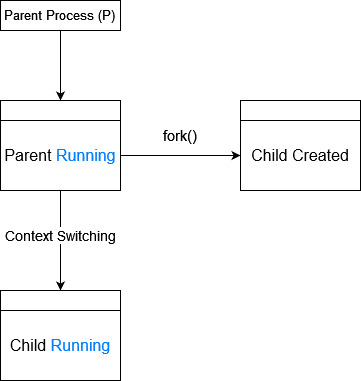
\includegraphics[width=0.75\textwidth]{assets/Forking-and-Context-Switching.jpg}
        \label{fig:diagram}
\end{figure}
\subsubsection {Parent Process}
    {Parent process} adalah proses yang memulai atau membuat proses lain. Dalam banyak sistem operasi, proses baru dibuat menggunakan sistem panggilan seperti fork() (di Unix/Linux). Parent process biasanya adalah proses yang sudah berjalan dan bertanggung jawab untuk memulai proses baru.
    Setelah memulai child process, parent process tetap bisa berjalan bersamaan dengan child process-nya atau bisa menunggu hingga child process selesai.

\subsubsection {Child Process}

\begin{itemize}
    
    \item{Child Process:} Child process adalah sebuah proses yang dihasilkan dari parent process. Child process ini merupakan salinan dari parent process, yang berarti pada saat pembuatannya, ia memiliki atribut dan konteks eksekusi yang sama dengan parent process-nya. Namun, meskipun child process diawali sebagai salinan, ia memiliki identitas yang unik dalam bentuk Process ID (PID) yang berbeda dari parent process-nya. Hal ini memungkinkan sistem operasi untuk membedakan antara parent dan child process dalam manajemen prosesnya.
    
    \item{Pewarisan Properti:} Child process seringkali mewarisi berbagai properti dari parent process. Properti-properti yang diwariskan dapat mencakup lingkungan eksekusi (environment), seperti variabel lingkungan dan pengaturan konfigurasi yang diperlukan untuk menjalankan proses, prioritas proses yang menentukan seberapa cepat atau lambat proses tersebut akan mendapatkan akses ke sumber daya sistem, serta akses file yang dibuka oleh parent process, memungkinkan child process untuk melanjutkan operasi pada file yang sama. Misalnya, jika parent process memiliki file terbuka untuk penulisan, child process dapat mewarisi akses ini dan melanjutkan operasi pada file yang sama.
    
    \item{Eksekusi Mandiri:} Setelah dibuat, child process dapat berjalan secara mandiri. Ini berarti bahwa ia tidak perlu selalu bergantung pada parent process untuk melanjutkan eksekusinya. Child process dapat menjalankan tugas-tugas yang berbeda dari parent process-nya, memungkinkan pemisahan kerja yang lebih efektif. Dalam beberapa kasus, child process akan menggunakan fungsi seperti exec() (di Unix/Linux) untuk menggantikan kode program yang diwarisinya dari parent dengan program baru yang benar-benar berbeda. Kemampuan ini memberikan fleksibilitas dalam sistem operasi untuk menjalankan berbagai tugas yang lebih kompleks dan terpisah, yang tidak harus bergantung pada program yang dijalankan oleh parent process. Sebagai contoh, dalam sebuah web server, parent process dapat membuat child process untuk menangani setiap permintaan klien secara mandiri, sehingga memungkinkan server untuk menangani beberapa klien sekaligus.
\end{itemize}

\subsubsection{Cara Parent dan Child Process Berinteraksi}

\begin{itemize}
    \item {Komunikasi Antarproses (IPC):} Dalam sistem operasi, parent dan child process dapat berkomunikasi satu sama lain melalui berbagai mekanisme Inter-Process Communication (IPC). Mekanisme ini memungkinkan pertukaran data atau sinyal antarproses. Beberapa metode umum IPC meliputi:

    
    {Pipe :} Sebuah saluran komunikasi satu arah di mana data dikirim dari satu proses ke proses lain dalam bentuk aliran byte. Ini memungkinkan parent process untuk mengirimkan data ke child process atau sebaliknya.
    
    {Shared Memory :} Parent dan child process dapat berbagi segmen memori yang memungkinkan mereka untuk membaca dan menulis data secara bersama-sama tanpa harus melakukan penyalinan data yang berlebihan.
    
    {Sinyal (Signal) :} Sinyal adalah bentuk komunikasi sederhana yang dapat digunakan oleh parent process untuk memberitahu child process mengenai suatu event, seperti perintah untuk menghentikan eksekusi atau melanjutkan eksekusi. Sinyal juga dapat digunakan oleh child process untuk mengirimkan informasi status kembali ke parent.
    
    \item {Status Child Process :} Parent process memiliki kemampuan untuk melacak status eksekusi child process. Salah satu cara untuk melakukan ini adalah dengan menggunakan panggilan sistem seperti wait() di Unix/Linux. Panggilan ini membuat parent process menunggu hingga child process selesai menjalankan tugasnya. Selama child process berjalan, parent process dapat memantau kapan child process selesai,lalu child process berakhir secara normal atau melalui penghentian yang tidak terduga. Setelah child process selesai, parent process dapat exit status dari child process, yang dapat memberikan informasi tentang bagaimana child process diselesaikan, apakah ada kesalahan atau tugas yang berhasil dijalankan.
    
    \item {Pewarisan Resource:} Saat child process dibuat, ia biasanya mewarisi resource yang digunakan oleh parent process. Resource ini dapat mencakup:

    {File Descriptors :} Child process mewarisi file yang sudah dibuka oleh parent process. Jika parent membuka file untuk dibaca atau ditulis, child process juga dapat melakukan operasi yang sama pada file tersebut tanpa harus membuka ulang.
    
    {Variable Lingkungan:} Child process sering kali mewarisi semua variabel lingkungan (environment variables) dari parent process. Variabel lingkungan ini digunakan untuk menentukan pengaturan sistem yang penting, seperti jalur pencarian untuk executable, informasi terkait pengguna, dan pengaturan regional.
   
    {Hak Akses:} Child process juga dapat mewarisi hak akses yang dimiliki oleh parent, seperti izin untuk mengakses file tertentu atau menggunakan resource perangkat keras. Namun, sering kali child process dapat berjalan dengan hak akses yang lebih rendah dari parent process untuk meningkatkan keamanan, seperti dijelaskan sebelumnya.
\end{itemize}

\subsubsection{Contoh di Unix/Linux}

\begin{itemize}
    \item Fungsi fork(): Pada sistem operasi berbasis Unix atau Linux, pembuatan child process dilakukan menggunakan fungsi fork(). Fungsi ini sangat penting dalam sistem operasi karena memungkinkan parent process untuk membuat salinan dirinya dalam bentuk child process. Ketika fork() dipanggil, sistem operasi membuat duplikat dari parent process, di mana child process baru mendapatkan salinan dari semua data yang dimiliki parent process, termasuk variabel, file descriptor, dan status eksekusi. Namun, meskipun child process merupakan duplikat, ia memiliki Process ID (PID) yang unik dan berbeda dari parent process. Dengan demikian, setelah fork(), kedua proses tersebut akan berjalan secara paralel atau bergantian, tergantung pada algoritma penjadwalan yang digunakan oleh sistem operasi.
    
    \item Status Child Process: Parent process memiliki kemampuan untuk melacak status eksekusi child process. Salah satu cara untuk melakukan ini adalah dengan menggunakan panggilan sistem seperti wait() di Unix/Linux. Panggilan ini membuat parent process menunggu hingga child process selesai menjalankan tugasnya. Selama child process berjalan, parent process dapat memantau kapan child process selesai, apakah child process berakhir secara normal atau melalui penghentian yang tidak terduga. Setelah child process selesai, parent process dapat mengambil exit status dari child process, yang dapat memberikan informasi tentang bagaimana child process diselesaikan, apakah ada kesalahan atau tugas yang berhasil dijalankan.
\end{itemize}

\subsubsection{Manfaat dan Penggunaan}

\begin{itemize}
    \item Keterpisahan tugas: Memisahkan tugas-tugas menjadi child process memungkinkan sistem operasi untuk mendistribusikan pekerjaan secara lebih efektif. Setiap child process dapat menangani tugas tertentu secara mandiri tanpa mengganggu eksekusi tugas lainnya. Hal ini memungkinkan sistem untuk menjalankan banyak proses secara bersamaan (multi-tasking), yang sangat penting dalam lingkungan yang sibuk atau intensif komputasi, seperti server web atau aplikasi pengolahan data skala besar. Dengan menggunakan banyak child process, beban kerja dapat dibagi sehingga mempercepat waktu respon dan meningkatkan efisiensi keseluruhan sistem. Selain itu, pembagian tugas ini membuat sistem lebih fleksibel dalam hal manajemen beban, di mana satu proses dapat dialihkan atau dihentikan tanpa memengaruhi proses lainnya, sehingga meningkatkan ketahanan sistem terhadap kegagalan.

    \item Keamanan: Dalam konteks keamanan, child process sering kali dijalankan dengan hak akses yang lebih terbatas dibandingkan dengan parent process-nya. Ini berarti child process tidak memiliki akses penuh ke seluruh sistem, tetapi hanya dapat mengakses sumber daya yang diizinkan oleh parent process atau sistem operasi. Pendekatan ini mengurangi risiko jika terjadi kesalahan atau kerentanan di dalam child process, karena dampaknya akan terbatas pada child process itu sendiri dan tidak akan menyebar ke seluruh sistem. Dengan isolasi yang ketat ini, child process yang rentan atau bermasalah tidak dapat merusak proses lain atau mengakses informasi yang tidak diizinkan, sehingga meningkatkan keamanan sistem secara keseluruhan, terutama dalam aplikasi yang melibatkan data sensitif atau akses jaringan yang luas, seperti perbankan online atau cloud computing.
\end{itemize}

\subsection{Introduction to Threads}
This section introduces the concept of threads and their relation to processes, covering:
\begin{itemize}
    \item Single-threaded vs. multi-threaded processes
    \item Benefits of multithreading
\end{itemize}

\begin{figure}[h]
    \centering
    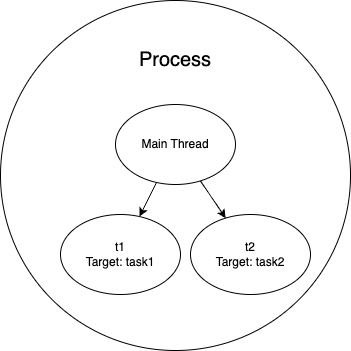
\includegraphics[width=0.5\textwidth]{/Users/khawaritzmi/Unhas/os_report_mid2024/b_class/asset/example.png}  % Sesuaikan nama file dan ukurannya
    \caption{Ini adalah gambar contoh dari multithreading.}
    \label{fig:contoh_gambar}
\end{figure}

Seperti yang terlihat pada Gambar \ref{fig:contoh_gambar}, inilah cara menambahkan gambar dengan keterangan.

\subsection{File Systems}
File systems provide a way for the operating system to store, retrieve, and manage data. This section explains:
\begin{itemize}
    \item File system structure
    \item File access methods
    \item Directory management
\end{itemize}

\subsection{Input and Output Management}
Input and output management is key for handling the interaction between the system and external devices. This section includes:
\begin{itemize}
    \item Device drivers
    \item I/O scheduling
\end{itemize}

\subsection{Deadlock Introduction and Prevention}
Explores the concept of deadlocks and methods for preventing them:
\begin{itemize}
    \item Deadlock conditions
    \item Deadlock prevention techniques
\end{itemize}

\subsection{User Interface Management}
This section discusses the role of the operating system in managing the user interface. Topics covered include:
\begin{itemize}
    \item Graphical User Interface (GUI)
    \item Command-Line Interface (CLI)
    \item Interaction between the user and the operating system
\end{itemize}

\subsection{Virtualization in Operating Systems}
Virtualization allows multiple operating systems to run concurrently on a single physical machine. This section explores:
\begin{itemize}
    \item Concept of virtualization
    \item Hypervisors and their types
    \item Benefits of virtualization in modern computing
\end{itemize}

\section{Assignments and Practical Work}
\subsection{Assignment 1: Process Scheduling}
Students were tasked with implementing various process scheduling algorithms (e.g., FCFS, SJN, and RR) and comparing their performance under different conditions.
\subsubsection{Group 1}
\begin{python}
    class Process:
    def __init__(self, pid, arrival_time, burst_time):
        self.pid = pid
        self.arrival_time = arrival_time
        self.burst_time = burst_time
        self.completion_time = 0
        self.turnaround_time = 0
        self.waiting_time = 0
\end{python}

\begin{table}[htbp] % Optional: For floating position
    \centering
    \begin{tabular}{|c|c|c|} % Defines number of columns and alignment (c = center, l = left, r = right). '|' creates vertical lines.
    \hline
    Header 1 & Header 2 & Header 3 \\ % Column headers
    \hline
    Row 1, Column 1 & Row 1, Column 2 & Row 1, Column 3 \\ % First row of data
    \hline
    Row 2, Column 1 & Row 2, Column 2 & Row 2, Column 3 \\ % Second row of data
    \hline
    \end{tabular}
    \caption{Your table caption} % Optional: For adding a caption
    \label{tab:your_label} % Optional: For cross-referencing the table
\end{table}

\subsection{Assignment 2: Deadlock Handling}
In this assignment, students were asked to simulate different deadlock scenarios and explore various prevention methods.

\subsection{Assignment 3: Multithreading and Amdahl's Law}
This assignment involved designing a multithreading scenario to solve a computationally intensive problem. Students then applied **Amdahl's Law** to calculate the theoretical speedup of the program as the number of threads increased.

\subsection{Assignment 4: Simple Command-Line Interface (CLI) for User Interface Management}
Students were tasked with creating a simple **CLI** for user interface management. The CLI should support basic commands such as file manipulation (creating, listing, and deleting files), process management, and system status reporting.

\subsection{Assignment 5: File System Access}
In this assignment, students implemented file system access routines, including:
\begin{itemize}
    \item File creation and deletion
    \item Reading from and writing to files
    \item Navigating directories and managing file permissions
\end{itemize}

\section{Conclusion}
The first half of the course introduced core operating system concepts, including process management, scheduling, multithreading, and file system access. These topics provided a foundation for more advanced topics to be covered in the second half of the course.

\begin{thebibliography}{9}

    \bibitem{Silberschatz2018}
    Silberschatz, A., Galvin, P. B., \& Gagne, G. (2018). \textit{Operating System Concepts} (10th ed.). Wiley.
    
    \bibitem{Kerrisk2010}
    Kerrisk, M. (2010). \textit{The Linux Programming Interface: A Linux and UNIX System Programming Handbook}. Journal Coders Press.
    
    \bibitem{Tanenbaum2014}
    Tanenbaum, A. S., \& Bos, H. (2014). \textit{Modern Operating Systems} (4th ed.). Pearson.
    
    \bibitem{Stallings2018}
    Stallings, W. (2018). \textit{Operating Systems: Internals and Design Principles} (9th ed.). Pearson.
    
    \end{thebibliography}

\end{document}